\newcommand\tab[1][1cm]{\hspace*{#1}}
\graphicspath{{images/}{images/logos/}}
\begin{frame}{Übersicht GUI}
	%\begin{center}
		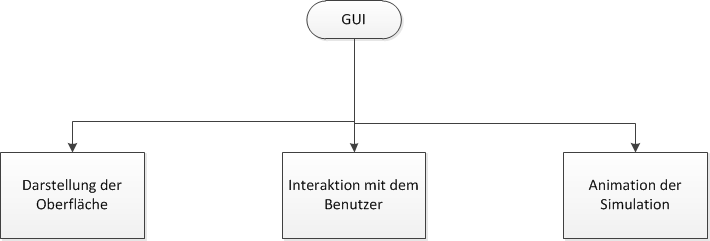
\includegraphics[width=300px,height=260px, keepaspectratio]{./model2.png}
	%\end{center}
\end{frame}

\begin{frame}{Darstellung der Oberfläche}
	\begin{center}
		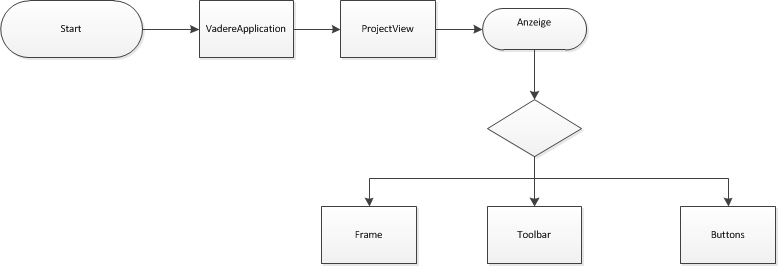
\includegraphics[width=300px,height=190px]{./model21.png}
	\end{center}
\end{frame}

\begin{frame}{Verwaltung der Actions}
	\begin{center}
		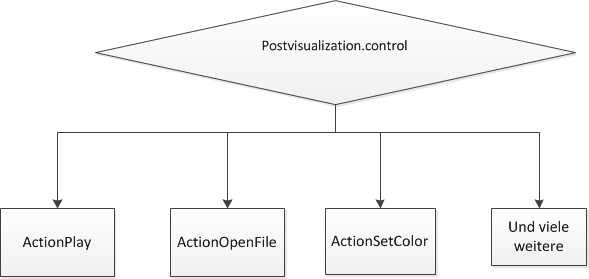
\includegraphics[width=250px,height=200px]{./model22a.png}
	\end{center}
\end{frame}


\begin{frame}{Verwaltung der Scenarios}
	\begin{center}
		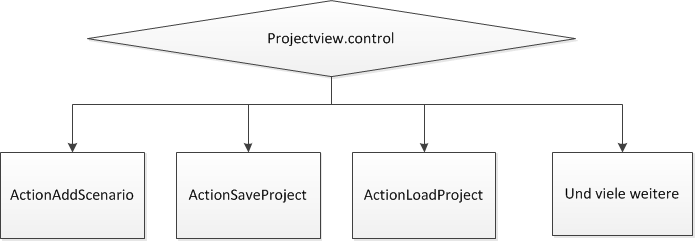
\includegraphics[width=300px,height=210px]{./model22b.png}
	\end{center}
\end{frame}


\begin{frame}{Zeichnen des Scenarios}
	\begin{center}
		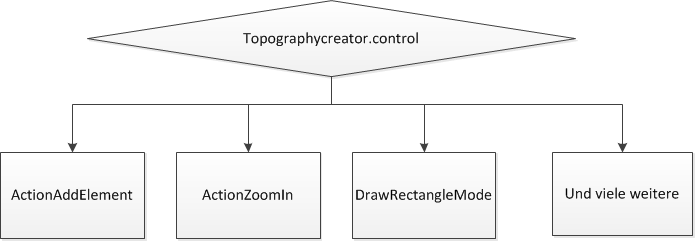
\includegraphics[width=300px,height=241px]{./model22c.png}
	\end{center}
\end{frame}


\begin{frame}{Animation der Simulation}
	\begin{center}
		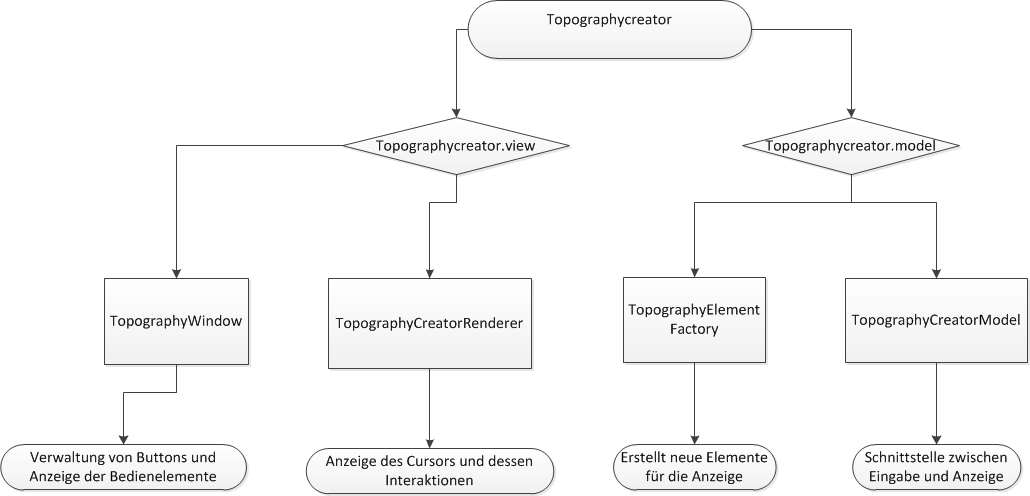
\includegraphics[width=300px,height=200px]{./model23a.png}
	\end{center}
\end{frame}

\begin{frame}{Zeichnen der Grafiken}
	\begin{center}
		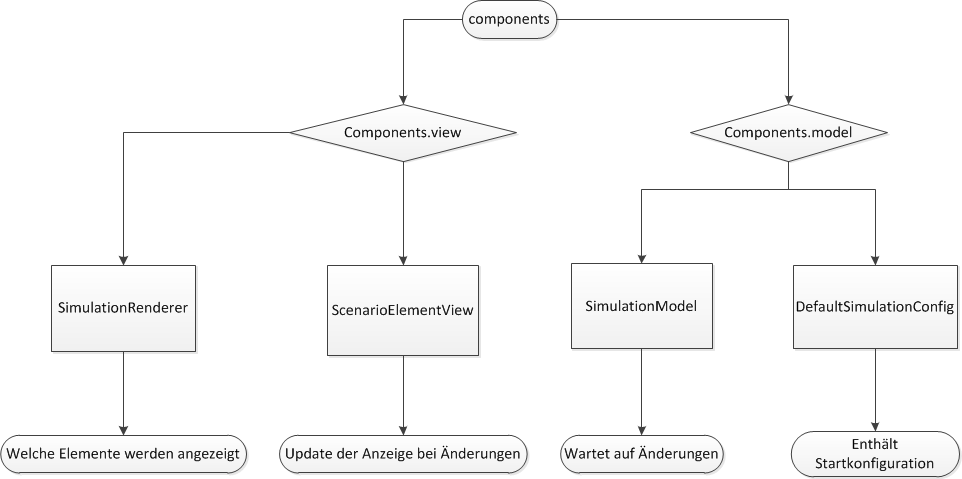
\includegraphics[width=300px,height=200px]{./model23b.png}
	\end{center}
\end{frame}


\begin{frame}{Button zu Horse}
	\begin{center}
		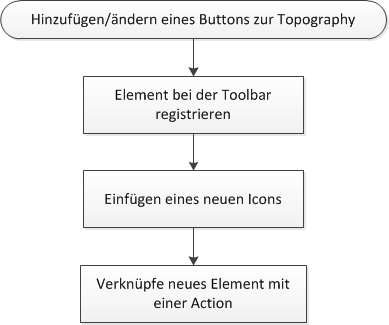
\includegraphics[width=300px,height=200px]{./model31.png}
	\end{center}
\end{frame}


\begin{frame}{Einbinden der Klasse Horse in GUI}
	\begin{center}
		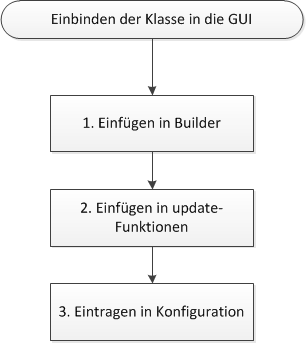
\includegraphics[width=300px,height=200px]{./model32a.png}
	\end{center}
\end{frame}


\begin{frame}{Einfügen in Builder}
	\begin{center}
		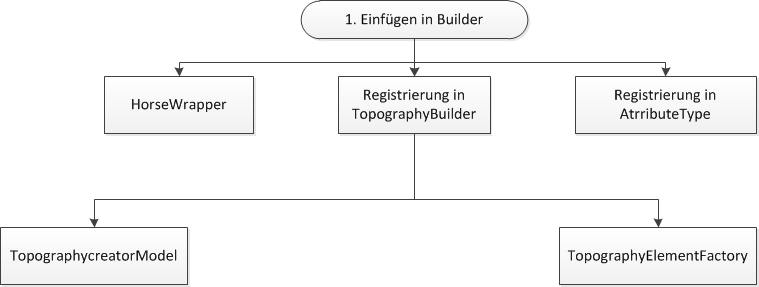
\includegraphics[width=300px,height=200px]{./model32b.png}
	\end{center}
\end{frame}

\begin{frame}{Einfügen in update - Funktionen}
	\begin{center}
		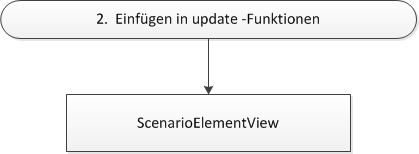
\includegraphics[width=300px,height=154px]{./model32c.png}
	\end{center}
\end{frame}

\begin{frame}{Eintragen in Konfiguration}
	\begin{center}
		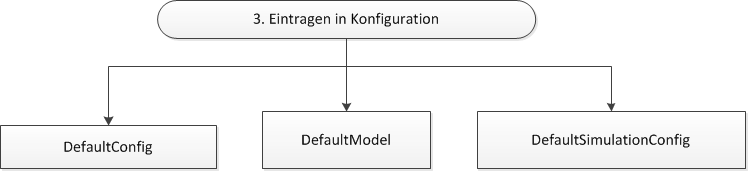
\includegraphics[width=300px,height=171px]{./model32d.png}
	\end{center}
\end{frame}


